%source mathadata
\vspace{0.2cm}
	\begin{minipage}{0.2\textwidth}
		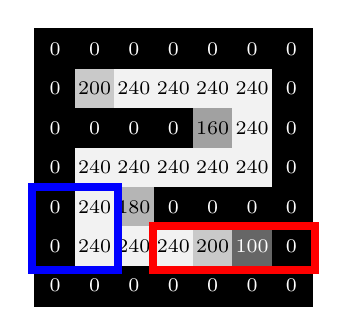
\begin{tikzpicture}[scale=0.5]
			\def\grid{
				{0,0,0,0,0,0,0},
				{0,200,240,240,240,240,0},
				{0,0,0,0,160,240,0},
				{0,240,240,240,240,240,0},
				{0,240,180,0,0,0,0},
				{0,240,240,240,200,100,0},
				{0,0,0,0,0,0,0},
			}                \foreach \row[count=\i from 0] in \grid {                \foreach \value[count=\j from 0] in \row {
					\pgfmathsetmacro{\gray}{int(100-\value/2.55)}
					\fill[black!\gray!white] (\j, -\i) rectangle ++(1, -1);
					\pgfmathsetmacro{\textcolor}{ifthenelse(\gray<50, "black", "white")}
					% réduire la taille : \small, \footnotesize, \scriptsize, \tiny
					\node[text=\textcolor] at (\j+0.5, -\i-0.5) {\scriptsize \value};                }
			}
			\draw[black, line width=0.5mm] (0, 0) rectangle (7, -7);
			\draw[blue, line width=1mm] (-0.1, -3.99) -- (2.1, -3.99)--(2.1,-6.1)--(-0.1,-6.1)--cycle;
			\draw[red, line width=1mm] (2.99, -4.99) -- (7.1, -4.99)--(7.1,-6.1)--(2.99,-6.1)--cycle;
		\end{tikzpicture}
	\end{minipage}\hfill \begin{minipage}{0.2\textwidth}
		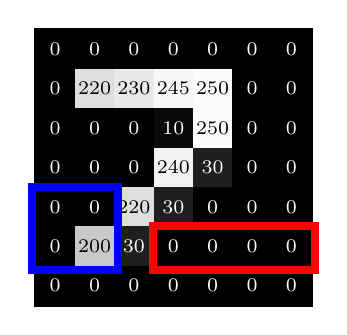
\begin{tikzpicture}[scale=0.5]
			\def\grid{
				{0,0,0,0,0,0,0},
				{0,220,230,245,250,0,0},
				{0,0,0,10,250,0,0},
				{0,0,0,240,30,0,0},
				{0,0,220,30,0,0,0},
				{0,200,30,0,0,0,0},
				{0,0,0,0,0,0,0},                }                \foreach \row[count=\i from 0] in \grid {                \foreach \value[count=\j from 0] in \row {
					\pgfmathsetmacro{\gray}{int(100-\value/2.55)}
					\fill[black!\gray!white] (\j, -\i) rectangle ++(1, -1);
					\pgfmathsetmacro{\textcolor}{ifthenelse(\gray<50, "black", "white")}
					\node[text=\textcolor] at (\j+0.5, -\i-0.5) {\scriptsize \value};
				}
			}
			\draw[black, line width=0.5mm] (0, 0) rectangle (7, -7);
			\draw[blue, line width=1mm] (-0.1, -3.99) -- (2.1, -3.99)--(2.1,-6.1)--(-0.1,-6.1)--cycle;
			\draw[red, line width=1mm] (2.99, -4.99) -- (7.1, -4.99)--(7.1,-6.1)--(2.99,-6.1)--cycle;            \end{tikzpicture}
	\end{minipage}\hfill \begin{minipage}{0.2\textwidth}
		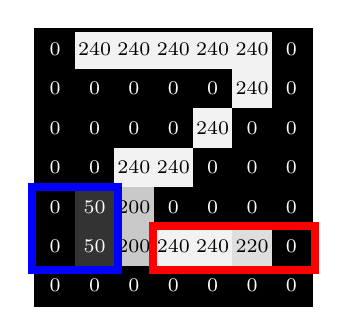
\begin{tikzpicture}[scale=0.5]
			\def\grid{
				{0,240,240,240,240,240,0},
				{0,0,0,0,0,240,0},
				{0,0,0,0,240,0,0},
				{0,0,240,240,0,0,0},
				{0,50,200,0,0,0,0},
				{0,50,200,240,240,220,0},
				{0,0,0,0,0,0,0},                }                \foreach \row[count=\i from 0] in \grid {                \foreach \value[count=\j from 0] in \row {                \pgfmathsetmacro{\gray}{int(100-\value/2.55)}
					\fill[black!\gray!white] (\j, -\i) rectangle ++(1, -1);
					\pgfmathsetmacro{\textcolor}{ifthenelse(\gray<50, "black", "white")}
					\node[text=\textcolor] at (\j+0.5, -\i-0.5) {\scriptsize \value};
				}
			}
			\draw[black, line width=0.5mm] (0, 0) rectangle (7, -7);
			\draw[blue, line width=1mm] (-0.1, -3.99) -- (2.1, -3.99)--(2.1,-6.1)--(-0.1,-6.1)--cycle;
			\draw[red, line width=1mm] (2.99, -4.99) -- (7.1, -4.99)--(7.1,-6.1)--(2.99,-6.1)--cycle;
		\end{tikzpicture}
	\end{minipage}\hfill \begin{minipage}{0.2\textwidth}
		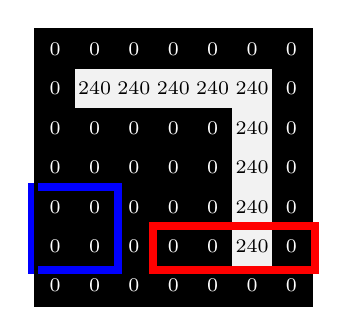
\begin{tikzpicture}[scale=0.5] \def\grid{
				{0,0,0,0,0,0,0},
				{0,240,240,240,240,240,0},
				{0,0,0,0,0,240,0},
				{0,0,0,0,0,240,0},
				{0,0,0,0,0,240,0},
				{0,0,0,0,0,240,0},
				{0,0,0,0,0,0,0}, } \foreach \row[count=\i from 0] in \grid { \foreach \value[count=\j from 0] in \row { \pgfmathsetmacro{\gray}{int(100-\value/2.55)} \fill[black!\gray!white] (\j, -\i) rectangle ++(1, -1); \pgfmathsetmacro{\textcolor}{ifthenelse(\gray<50, "black", "white")} \node[text=\textcolor] at (\j+0.5, -\i-0.5) {\scriptsize \value}; } }\draw[blue, line width=1mm] (-0.1, -3.99) -- (2.1, -3.99)--(2.1,-6.1)--(-0.1,-6.1)--cycle;
			\draw[black, line width=0.5mm] (0, 0) rectangle (7, -7);
			\draw[red, line width=1mm] (2.99, -4.99) -- (7.1, -4.99)--(7.1,-6.1)--(2.99,-6.1)--cycle; \end{tikzpicture}
	\end{minipage}

	\begin{multicols}{2}
		On utilise deux caractéristiques $\color{red}{x}$ et $\color{blue}{y}$ pour mieux différencier les images de 2 et de 7. On note $\color{red}{x}$ la moyenne des pixels dans le rectangle rouge et $\color{blue}{y}$ la moyenne des pixels dans le rectangle bleu.
		\begin{MADenumerate}
			\item Calculer les deux caractéristiques $(\color{red}{x} ~;~\color{blue}{y})$ pour chacune des quatre images.

			\item Pour chaque image, représenter les couples $(\color{red}{x} ~;~\color{blue}{y})$ sous la forme d'un point dans le plan appelé \textbf{point associé} à l'image avec deux couleurs différentes selon que l'image représente un 2 ou un 7.
		\end{MADenumerate}
		%             \columnbreak
		\begin{tikzpicture}[scale=0.9]
			\begin{axis}[
					name=plotA,
					axis lines=middle,
					ymajorgrids=true,
					xmajorgrids=true,
					xmin=-1.1,
					xmax=180,
					ymin=-0.1,
					ymax=180,
					xtick={20,40,...,180},
					ytick={20,40,...,180},
					xlabel={\Large {\color{red} $x$}},
					xlabel style={at={(axis description cs:1.02,-0.1)}, anchor=north},
					ylabel={\color{blue}{\Large $y$}},
					ylabel style={at={(axis description cs:-0.2,1.02)}, anchor=west},
					scatter/classes={
							A={mark=square*,mark size = 2pt,draw=blue, fill = BleuCeladon},
							B={mark=*,mark size = 2pt,draw=black, fill = OrangeCarotte},
							C={mark=square*,mark size = 4pt,draw=blue, fill = BleuCeladon},
							D={mark=*,mark size = 4pt,draw=black, fill = OrangeCarotte}
						}
				]
				%\clip(-0.2,-0.2) rectangle (8,6);
				\addplot[scatter,only marks,scatter src=explicit symbolic,opacity=0]
				coordinates {
						(0,115)[A]
						(140,145)[A]
						(155,60)[A]
						(0,40)[B]
						(51,50)[B]
						(62,5)[B]
						(135,120)[C]
						(0,50)[D]
						(175,25)[C]
						(60,0)[D]
					};
			\end{axis}
			\draw (0,0) node[below left]{\footnotesize $O$};
		\end{tikzpicture}
	\end{multicols}

	\begin{MADenumerate}[3]
		\item Placer les 6 points associés aux images du tableau ci-dessous dans le repère.
		\begin{center}
			\hspace{-1.4cm}
			\begin{tabular}{|c|*{3}{>{\columncolor{BleuCeladon!20}}c|}*{3}{>{\columncolor{OrangeCarotte!20}}c|}}
				\hline
				\rowcolor{floralwhite}Image
				                                              & \includegraphics[width=0.09\linewidth,clip,trim=0cm 4cm 0cm 0cm]{images/zone_2_cara_image6.png} & \includegraphics[width=0.09\linewidth,clip,trim=0cm 4cm 0cm 0cm]{images/zone_2_cara_image5.png} & \includegraphics[width=0.09\linewidth,clip,trim=0cm 4cm 0cm 0cm]{images/zone_2_cara_image4.png} & \includegraphics[width=0.09\linewidth,clip,trim=0cm 4cm 0cm 0cm]{images/zone_2_cara_image3.png} & \includegraphics[width=0.09\linewidth,clip,trim=0cm 4cm 0cm 0cm]{images/zone_2_cara_image2.png}
				                                              & \includegraphics[width=0.09\linewidth,clip,trim=0cm 4cm 0cm 0cm]{images/zone_2_cara_image1.png}
				\\\hline

				Chiffre                                       & 2                                                                                               & 2                                                                                               & 2                                                                                               & 2                                                                                               & 2                                                                                               & 7           \\\hline
				$\left(\color{red}{x};\color{blue}{y}\right)$ & $(0 ~;~115)$                                                                                    & $(140 ~;~145)$                                                                                  & $(155 ~;~60)$                                                                                   & $(0 ~;~40)$                                                                                     & $(51 ~;~50)$                                                                                    & $(62 ~;~5)$ \\\hline
			\end{tabular}
		\end{center}
		\item Tracer une droite qui sépare au mieux les points associés aux images de 2 et de 7.
		\item Avec les informations à disposition, que dire d'une image de caractéristiques $(135 ~;~120)$ ?
	\end{MADenumerate}
